\documentclass[10pt,a4paper]{article}
\usepackage[T1]{fontenc}
\usepackage[utf8]{inputenc}
\usepackage{lmodern,graphicx,booktabs,longtable,array,amsmath,amssymb,float}
\usepackage[margin=18mm]{geometry}
\usepackage[numbers,sort&compress]{natbib}
\usepackage[hyphens]{url}
\usepackage[hidelinks]{hyperref}
\IfFileExists{microtype.sty}{\usepackage{microtype}}{}
\IfFileExists{caption.sty}{\usepackage[font=small,labelfont=bf]{caption}}{}
\setlength{\parskip}{4pt}
\setlength{\parindent}{0pt}
\setlength{\emergencystretch}{3em}
\setlength{\textfloatsep}{12pt}
\setlength{\intextsep}{12pt}
\setlength{\abovecaptionskip}{6pt}
\renewcommand{\topfraction}{.92}
\renewcommand{\bottomfraction}{.88}
\renewcommand{\textfraction}{.06}
\renewcommand{\floatpagefraction}{.82}
\widowpenalty=10000
\clubpenalty=10000
\makeatletter
\setlength{\@fptop}{0pt}
\makeatother
\newcommand{\figref}[1]{Fig.~\ref{fig:#1}}
\title{A common BSA--serum equation for EASI estimation in a Chinese atopic dermatitis cohort}
\author{}
\date{}
\begin{document}
\maketitle
\begin{abstract}
\textbf{Background:} Connecting serum inflammation with clinical severity requires a practical calculation that remains interpretable across treatment and follow-up. We evaluated a common Eczema Area and Severity Index (EASI) equation within a Chinese treat-to-target cohort.

\textbf{Methods:} We examined clinical outcomes and all 23 serum markers under dupilumab and two initial abrocitinib doses, adjusting treatment comparisons for measured baseline differences. A model-development procedure using nominal-visit-matched affected body surface area (BSA), CCL17, CCL26 and IL-5 was developed with baseline/week-12 observations using nested patient-level validation and applied at week 24. Individual estimates, within-person changes and EASI75 identification were evaluated separately.

\textbf{Results:} Clinical comparisons included 163 patients; EASI estimation included 316 visits from 160 patients. Clinical control improved alongside treatment-dependent molecular changes. The selected four-input equation required no treatment label or previous score; performance estimates describe the nested development procedure. Mean absolute error (MAE) at baseline/weeks 12/24 was 3.19/1.30/1.19, with Spearman correlations of 0.918/0.927/0.904. Follow-up errors were within two points in 84.3\% and 82.0\% of predictions. MAEs for within-person changes over baseline--week 12, baseline--week 24 and weeks 12--24 were 3.87, 3.47 and 1.49. EASI75 sensitivity at weeks 12/24 was 76.5\%/86.1\%, with specificity of 98.6\%/96.2\%.

\textbf{Conclusions:} The BSA--serum development procedure gave close follow-up EASI estimates and tracked changes within this cohort. Molecular added accuracy was not established, and baseline severe disease remained the main accuracy boundary. These results support independent evaluation of this restricted-input research measure across the severity range.

\end{abstract}
\textbf{Keywords:} atopic dermatitis; biomarkers; EASI; longitudinal estimation; treat-to-target.
\section{Introduction}
Atopic dermatitis treatment must improve visible skin disease, itch and the burden of living with eczema. Treat-to-target frameworks bring these complementary outcomes into treatment decisions, including early symptom relief and later disease control.\citep{williams2022home,debruin2021t2t,zhao2026t2t} A practical severity estimate should remain interpretable as treatment changes and should capture how an individual patient's condition changes, rather than only distinguish groups with different average severity.

Serum markers offer a link between clinical activity and inflammation. The p-EASI approach combines CCL17, IL-22 and soluble IL-2 receptor, with different coefficients before and during treatment.\citep{thijs2017} Subsequent studies reported Spearman correlations of 0.71 during cyclosporin treatment and 0.67 during dupilumab treatment.\citep{thijs2019,bakker2020} These studies established a practical precedent for converting blood measurements into Eczema Area and Severity Index (EASI) units. Applying such a calculation in another setting also requires agreement with individual scores, compatible assays and evaluation across the severity range.\citep{luijken2020,riley2024validation}

EASI combines the extent of affected skin with lesion intensity.\citep{hanifin2022,home_easi} A small-input equation combining affected body surface area (BSA) and serum measurements could offer a common calculation without separate rules for each drug or treatment phase. BSA supplies the clinical extent component; the serum panel supplies molecular information. We evaluated it as a research readout of recorded EASI at the visit, with separate tests of individual change and molecular added accuracy. Measured itch, quality of life and safety remained complementary clinical assessments.

We investigated these questions in a Chinese cohort receiving dupilumab or two initial abrocitinib doses. We first established the clinical and molecular context, retaining all 23 measured serum markers and accounting for baseline differences and later treatment changes. We then developed a common BSA--serum equation, evaluated individual estimates and changes using patient-level validation, and examined unchanged published p-EASI formulas as a separate local-application comparison.

\section{Methods}
\subsection{Study population and clinical assessment}
We analysed longitudinal records from a Chinese observational treat-to-target project at CAMS and Huashan. The supplied protocol specified Hanifin--Rajka diagnosis and eligibility for systemic treatment. Actual screening implementation and recruitment dates were not recoverable from a verified screening register. Systemic treatment was clinician directed. Initial regimens were dupilumab, abrocitinib 100 mg or abrocitinib 200 mg; later dose, interval and regimen changes were recorded separately. Clinical comparisons included patients aged at least 12 years with an unambiguous initial regimen. Adult Dermatology Life Quality Index (DLQI) analyses required age at least 18.

Clinical outcomes were the recorded EASI, peak pruritus numerical rating scale (PP-NRS), Investigator Global Assessment (IGA), DLQI, BSA and SCORAD, with IgE and eosinophil measurements. Reporting visits were W0/W2/W4/W12/W24 for PP-NRS, W0/W12/W24 for IgE and W0/W4/W12/W24 for other measures. Records were linked by patient and nominal visit. The exact IGA and questionnaire versions, PP-NRS recall window and calendar-day clinical/serum matching require source confirmation. Source discrepancies were audited without substituting imputed clinical outcomes.

\subsection{Clinical framework, targets and treatment pathways}
Project materials describe evidence review, a two-round questionnaire procedure and a planned agreement criterion of at least 75\%. They report 49 returned questionnaires, without original ballots or round-specific agreement results. We transcribed the September framework and operationalized its targets on recorded scores (Fig.~\ref{fig:Figure1}). Its exact approved and prospectively implemented version remains unverified; this analysis does not validate a new consensus or the effectiveness of the management strategy.

The week-2 target was PP-NRS $\leq4$. At week 4, the physician target was EASI50 or an IGA decrease of at least two points, and the patient target was PP-NRS $\leq4$ or adult DLQI $\leq10$. At week 12, these were EASI75 or IGA 0/1, and PP-NRS 0/1 or adult DLQI $\leq4$. Week 24 additionally allowed EASI $\leq5$ in the physician domain. Both domains were required for the combined target. These investigator-defined targets were kept distinct from newer low-disease-activity and remission definitions.\citep{merola2026iec}

Each rate used its own evaluable denominator and Wilson 95\% confidence interval. EASI percentage responses required positive observed baseline EASI. A PP-NRS decrease of at least four points required observed baseline PP-NRS $\geq4$ and an observed follow-up score; lower or missing baseline values were excluded from that endpoint. Missing components remained unknown unless another observed component determined the logical result. Below age 18, adult DLQI was treated as unknown: a positive itch component establishes the patient target, whereas a negative itch component alone leaves it unknown. Group comparisons retained initial treatment after subsequent changes. Separate maintenance analyses classified week-12 response and later reduction pathways, then examined observed week-24 EASI75 with explicit missing-outcome bounds. Reduction was not reassigned to an earlier visit; uncertain assessment/decision timing was retained. These descriptive pathways address treatment changes without treating a response-selected maintenance group as randomized.\citep{iche9r1}

\subsection{Serum measurements}
Source laboratory reports described Luminex and MSD serum assays, including the LXSAHM-13 panel on Luminex-200 and K15067M-1/K15067M-2 kits on SQ120, using 50-$\mu$L serum and twofold dilution. All 23 measured markers were included. Analyses used positive numeric integration-export concentrations recorded in pg/mL, transformed to log$_2$ once without an additional dilution correction. The twofold laboratory dilution describes sample preparation; its correction in the export and validated quantification limits require source confirmation. Censoring strings and nonpositive values were not treated as measured positive concentrations. An IL-5 calibration-bound sensitivity analysis and detailed assay provenance are provided in the Supplementary Methods; software calibration limits were distinguished from validated quantification limits.

Molecular changes were calculated within patient for W0--W12, W12--W24 and W0--W24 before summarization. Three-visit displays additionally held the patient set fixed within each marker and treatment. This separates individual change from shifts in the patients observed at each visit.

\subsection{EASI estimation and validation}
Eligible model visits required age at least 12, observed EASI and BSA, and positive observed CCL17, CCL26 and IL-5. This three-marker panel was fixed from earlier exploratory work. Development used W0/W12; W24 was excluded from fitting and selection. As W24 had been examined in previous project analyses, it represents within-cohort temporal application, not untouched external validation.

A repeated five-fold patient-level outer validation with three-fold inner validation selected among three common structures and ridge penalties. All records from a patient stayed in one outer fold, preprocessing used training data only, and patients received equal total fitting weight. Full-development selection yielded a formula in which BSA multiplies a molecular component. Its rounded display is
\begin{align*}
\widehat{\mathrm{EASI}}\ \approx\ 
\operatorname{clip}_{[0,72]}\Bigl\{\frac{\mathrm{BSA}}{100}
\bigl[&51.27+0.98\log_2(\mathrm{CCL17})\\
&+0.96\log_2(\mathrm{CCL26})
-0.83\log_2(\mathrm{IL\mbox{-}5})\bigr]\Bigr\}.
\end{align*}
BSA is entered from 0 to 100 and concentrations use the development export's recorded pg/mL numerics, with the logarithm applied once. Here, clip bounds the result to 0--72, and log$_2$ is the base-two logarithm. The project label Skin inflammation score refers here to this hybrid EASI estimate, not a separately calibrated blood-only inflammation scale. The calculator retains full-precision parameters; the displayed approximation differed from final-equation predictions by less than 0.08 EASI points in this dataset. Threshold decisions use the precise calculator. Treatment, stage, time and previous scores are not inputs. Reported primary performance evaluates the nested selection procedure; it is not the apparent fit of this final equation.

Primary assessment used MAE with patient bootstrap intervals conditional on the saved held-out predictions; these intervals did not repeat model selection or fitting. This internal validation does not include the earlier selection of the marker panel. Additional measures were RMSE, signed error, Spearman correlation, Lin's concordance correlation and proportions within one or two EASI points. Repetition-specific metrics were calculated before averaging. Severity strata and centre/treatment holdouts assessed where performance varied. A separate refitting sensitivity removed development visits with complete regional scores whose sum differed from recorded total EASI by more than 0.15 points. It retained the original patient folds and outcomes and repeated inner selection; it tested exclusion robustness without correcting either clinical reference. Monitoring used estimated and observed changes within the same patient, repetition and fold; response classification used the corresponding estimated or observed scores at both ends of the interval. Matched controls included BSA alone and the three markers alone. Primary paired comparisons used the nested procedure; fixed-structure comparisons were labelled separately. Published p-EASI coefficients were applied unchanged as a source-table sensitivity analysis, using local IL2RA as an unbridged soluble IL-2 receptor proxy and retaining raw and matched-clipping results. Different inputs and unverified assay equivalence preclude a model-superiority claim.\citep{thijs2017,thijs2019,bakker2020} PP-NRS, adult DLQI and recorded IGA were fitted independently with target-appropriate regression or ordinal models using the same restricted inputs.

\subsection{Statistical analysis}
Patients were the independent units. Overall clinical trajectories showed means with 95\% intervals; treatment-specific observations showed medians and interquartile ranges. Continuous treatment comparisons used baseline-outcome adjustment, treatment-by-visit terms, age, sex, BMI and centre, generalized overlap weights and patient-cluster robust covariance. Weights target overlap in baseline treatment probabilities. Reported outcome contrasts are baseline-weighted associations among patients with that endpoint observed. Selective endpoint observation can therefore change the represented population and its covariate balance.\citep{lili2019} Weighted target contrasts used patient bootstrap intervals with propensity refitting. A W2 sensitivity additionally included baseline PP-NRS, comparing models on the same baseline-itch-complete cohort. Endpoint-specific balance, effective sample sizes and both weighted and unweighted missing-outcome bounds were retained; weighting did not correct informative follow-up loss. IgE/eosinophil models used log$(1+x)$ and back-transformation. The analyses estimate adjusted observational associations.

Unadjusted target comparisons used conditional Monte Carlo three-group tests and pairwise Fisher tests; the three pairwise contrasts within each endpoint/visit formed a Holm family. Molecular paired sign-flip tests used Benjamini--Hochberg adjustment over 23 markers, three treatments and three windows. Between-treatment molecular changes additionally adjusted for starting concentration and clinical baseline variables. Estimates based on fewer than five pairs were descriptive. Balance, effective sample size and common support were examined. Exact tests, numerical settings, model diagnostics, regional analyses and additional targets are detailed in the Supplementary Methods. Analyses used Python 3.9.6; dependency versions, code, data-access conditions and reproduction logs accompany the package. Reporting follows relevant STROBE and TRIPOD+AI domains.\citep{vonelm2007strobe,collins2024tripod}

\section{Results}
\subsection{Clinical framework and analysis populations}
The source framework combined at least one physician criterion with one patient criterion at W4, W12 and W24; W2 assessed itch alone (Fig.~\ref{fig:Figure1}). We used these stage-specific rules to calculate recorded-score targets. The serum-assisted EASI readout was evaluated as a parallel research measure and did not determine dose-reduction decisions.

\begin{figure}[!htbp]
\centering
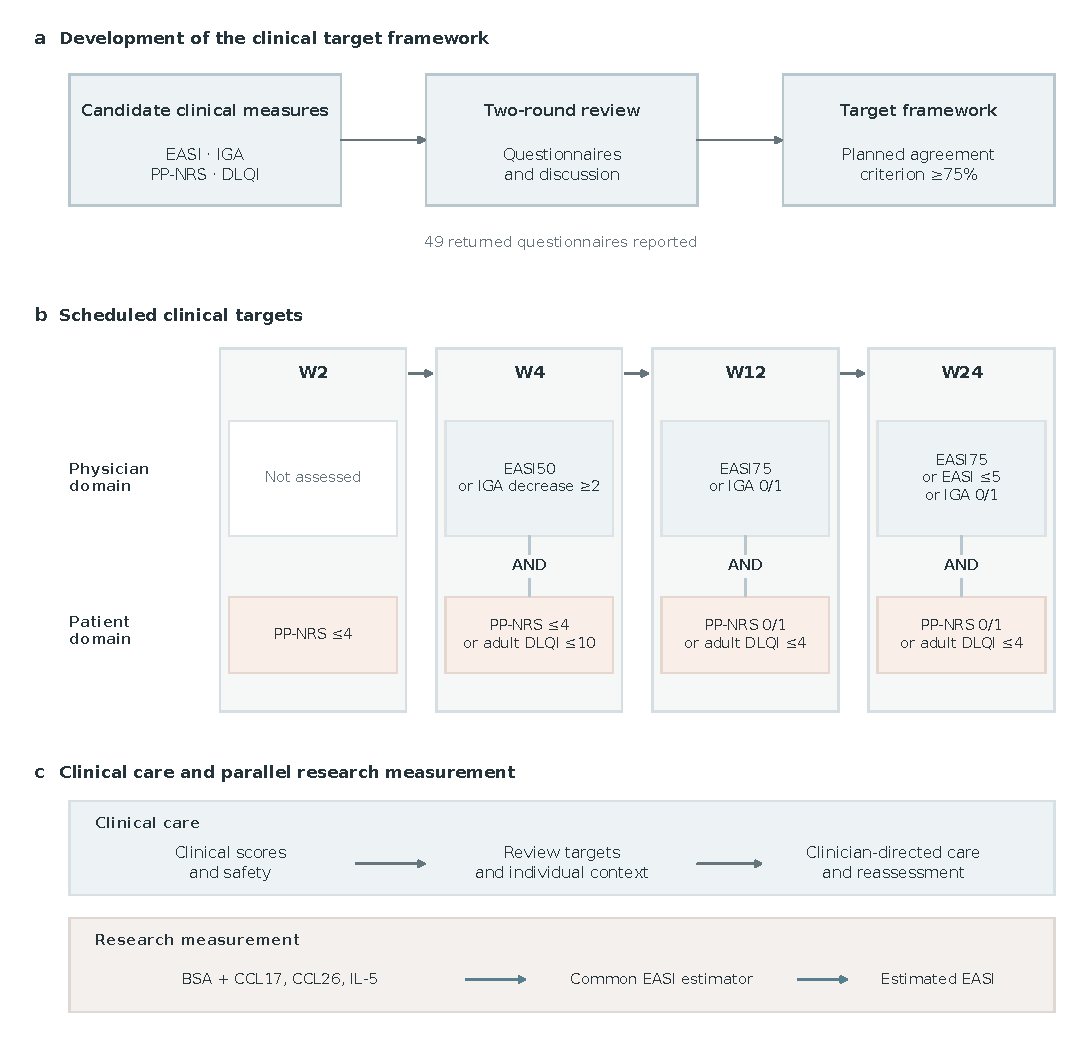
\includegraphics[width=\linewidth,height=.72\textheight,keepaspectratio]{figures/Figure1.pdf}
\caption{\textbf{Source framework, clinical targets and the research readout.} a, The project development summary describes candidate measures, a two-round questionnaire procedure and a planned $\geq$75\% agreement criterion, and reports 49 returned questionnaires. Original ballots and round-specific agreement results are unavailable; this is not a newly verified consensus experiment. b, The operational target schedule follows the source framework; milestone positions are schematic rather than time-scaled. EASI50/75 denotes at least 50\%/75\% improvement from positive observed baseline EASI. IGA decrease $\geq$2 is change from baseline; 0/1 denotes an observed grade or score of 0 or 1. OR applies within a domain and AND across domains. W2 is an itch-only target, not a combined physician-patient target. Adult DLQI requires age $\geq$18. Missing components use three-valued logic; adult DLQI is unknown below age 18. The IGA instrument and approved, implemented framework version require confirmation; these are exploratory recorded-score targets. c, Clinical assessment supports clinician-directed management. The BSA-serum readout is a parallel research addition, with clinical decision use untested. It does not replace examination, symptoms, quality of life or safety review. The cohort does not test framework effectiveness. Detailed definitions and provenance are provided in the Supplementary Methods.}\label{fig:Figure1}
\end{figure}

The clinical comparison included 163 patients: 65 started dupilumab, 56 abrocitinib 100 mg and 42 abrocitinib 200 mg. Median baseline EASI was 15.20, 11.70 and 19.35, respectively; age, sex and BMI also differed (Table~\ref{tab:baseline}). Clinical treatment comparisons and linked-serum modelling used separate eligibility rules. Their populations and overlap are shown in Supplementary Fig.~S37.

\begin{table}[!htbp]
\centering\footnotesize
\caption{Baseline characteristics of the clinical comparison population.}\label{tab:baseline}
\begin{tabular}{p{45mm}rrr}\toprule
 & Dupilumab & Abrocitinib 100 mg & Abrocitinib 200 mg \\ 
 & (n=65) & (n=56) & (n=42) \\ \midrule
Age, years & 54.0 (29.0--71.0) & 37.5 (22.0--52.0) & 24.5 (19.0--46.8) \\ 
BMI, kg/m$^2$ & 23.0 (21.0--26.0) & 22.4 (20.2--24.3) & 23.6 (21.4--26.0) \\ 
Male sex, n/N (\%) & 36/65 (55.4) & 27/56 (48.2) & 35/42 (83.3) \\ 
EASI & 15.2 (11.9--21.6) & 11.7 (7.7--17.3) & 19.4 (9.6--27.8) \\ 
PP-NRS & 8.0 (7.0--9.0) & 7.0 (5.5--8.0) & 7.0 (5.0--9.8) \\ 
\quad {\scriptsize Available n} & {\scriptsize 65} & {\scriptsize 55} & {\scriptsize 42} \\ 
IGA, recorded grade & 4.0 (3.0--4.0) & 3.0 (3.0--4.0) & 4.0 (3.2--4.8) \\ 
Adult DLQI & 15.0 (10.5--21.0) & 10.5 (7.0--15.2) & 15.0 (10.2--21.8) \\ 
\quad {\scriptsize Available n} & {\scriptsize 47} & {\scriptsize 32} & {\scriptsize 34} \\ 
BSA, \% & 23.0 (17.0--37.0) & 16.0 (10.0--25.2) & 25.0 (15.5--36.2) \\ 
SCORAD & 50.0 (43.2--59.4) & 48.1 (40.4--54.2) & 58.1 (48.7--72.6) \\ 
\quad {\scriptsize Available n} & {\scriptsize 65} & {\scriptsize 44} & {\scriptsize 41} \\ 
Eosinophils, recorded units & 0.2 (0.1--0.4) & 0.3 (0.1--0.6) & 0.5 (0.3--0.7) \\ 
\quad {\scriptsize Available n} & {\scriptsize 34} & {\scriptsize 51} & {\scriptsize 38} \\ 
IgE, recorded units & 200.0 (57.2--741.2) & 214.7 (71.0--626.0) & 700.0 (57.6--5000.0) \\ 
\quad {\scriptsize Available n} & {\scriptsize 62} & {\scriptsize 41} & {\scriptsize 37} \\ 
\bottomrule\end{tabular}
\par\small\raggedright Values are median (interquartile range), unless stated otherwise. Adult DLQI is restricted to age $\geq18$. IGA is retained on the recorded scale pending instrument confirmation. The column-header n applies unless an available n is shown. Missing values are not filled.\end{table}

\subsection{Clinical responses differed across initial treatment groups}
Clinical activity decreased and patients reached the successive treatment targets (Fig.~\ref{fig:Figure2}). At week 2, PP-NRS was at most 4 in 15/27 evaluable dupilumab recipients, 34/37 receiving initial abrocitinib 100 mg and 33/36 receiving initial abrocitinib 200 mg. The adjusted 100 mg--dupilumab difference in this early itch-target rate was 41.7 percentage points (95\% CI, 15.1--69.4; Holm-adjusted $P=0.0095$); adding baseline itch gave 41.4 points (13.0--66.8). W2 itch was unavailable for 38/65, 19/56 and 6/42 patients, respectively, so these available-case associations remain sensitive to follow-up selection. Weighted worst-case bounds at W2 were 19.4--82.0\% for dupilumab and 76.0--94.8\% for A100, allowing the contrast to reverse under extreme assignments of missing outcomes. These are sensitivity bounds, not confidence intervals. At week 24, the combined physician- and patient-reported target was reached by 26/36 (72.2\%), 22/24 (91.7\%) and 20/23 (87.0\%), respectively. Allowing all unknown outcomes to fail or succeed gave W24 combined-target bounds of 40.0--84.6\%, 39.3--96.4\% and 47.6--92.9\%. All specified clinical trajectories, component targets and exact denominators are retained in Supplementary Figs.~S1--S4, S15 and S22--S25.

\begin{figure}[!htbp]
\centering
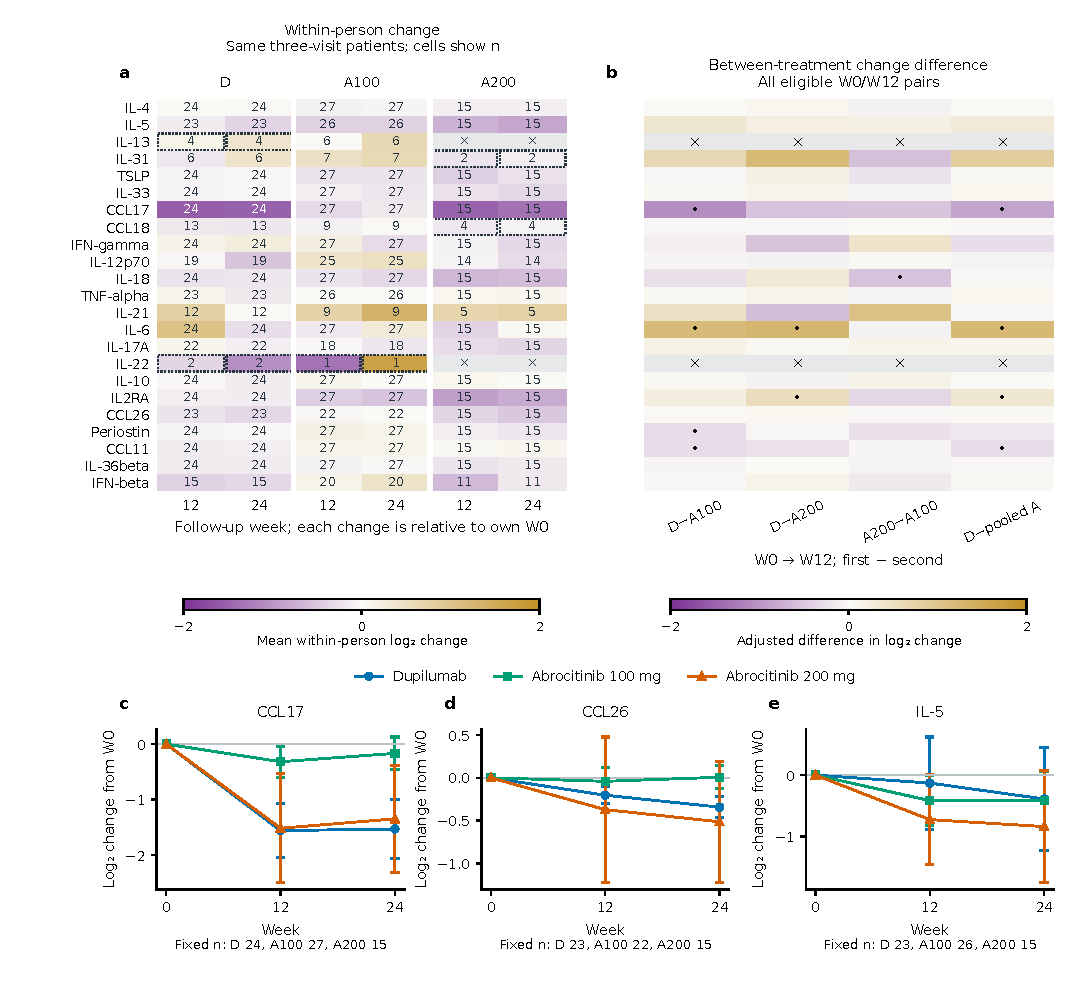
\includegraphics[width=\linewidth,height=.72\textheight,keepaspectratio]{figures/Figure2.pdf}
\caption{\textbf{Clinical course, response depth and target attainment.} a--c, Observed EASI, peak-pruritus numerical rating scale (PP-NRS) and adult Dermatology Life Quality Index (DLQI) medians with interquartile bands by initial treatment. Adult DLQI requires age $\geq$18. d--f, Observed EASI50/75/90 response rates at W4/W12/W24, with Wilson 95\% confidence intervals; response requires positive observed baseline EASI. Counts are in D/A100/A200 order, aligned to actual visits except the separately headed PP-NRS visit table. Lines describe available-case summaries, which need not retain the same patients over time. g, Observed stage-specific target rates with Wilson intervals and achieved/evaluable counts. W2 uses PP-NRS $\leq$4; later combined targets require a physician and a patient criterion, as defined in Fig. 1. Stage criteria differ, so these points are not joined. Missing outcomes remain unknown rather than observed failures. h, EASI differences from the common-reference generalized-overlap-weighted model, adjusted for baseline EASI, age, sex, BMI and centre, with patient-cluster-robust 95\% confidence intervals. Negative values favour the first named group for lower EASI; colour distinguishes W12/W24. D, dupilumab; A100/A200, initial abrocitinib 100/200 mg. Treatment was clinician directed, and later regimens could change. These are initial-strategy associations, not randomized fixed-dose effects. Remaining outcomes, IGA composition, actual regimens, missing-outcome bounds and complete adjusted target contrasts are retained in the supplement.}\label{fig:Figure2}
\end{figure}

The lower observed EASI in the 100 mg group did not persist as a clear dose-group difference after baseline adjustment. The adjusted 100-minus-200 mg difference was 0.62 points at week 12 (95\% CI, $-2.08$ to 3.33) and 0.34 at week 24 ($-1.10$ to 1.77). Weighting improved full-cohort baseline balance, although residual imbalance remained in endpoint-specific available-case samples (Supplementary Fig.~S38). These comparisons describe initial treatment under subsequent clinical management, including later regimen changes. Three W0 regimen entries conflicted with the initial-dose label and were retained as unresolved source conflicts. Recorded exposure composition and post-response reduction pathways are shown separately (Supplementary Figs.~S16--S17 and S39). Safety-related documentation through W24 was available for 27/65, 20/56 and 19/42 patients, respectively (Supplementary Table~S3). These counts describe note availability; event incidence, severity and event-time treatment attribution were not adjudicated.

\subsection{Molecular trajectories differed across treatment courses}
All 23 measured serum markers were retained, including CCL18, IL-13, IL-22 and IL-31. The W0/W12/W24 profiles showed treatment-dependent molecular changes alongside clinical improvement (Fig.~\ref{fig:Figure3}). Fixed three-visit displays used the same patients within each marker and treatment; the complete window analyses used all available pairs. Thus, differences in their sample sizes reflect distinct eligible sets, rather than changes to the measurements.

\begin{figure}[!htbp]
\centering
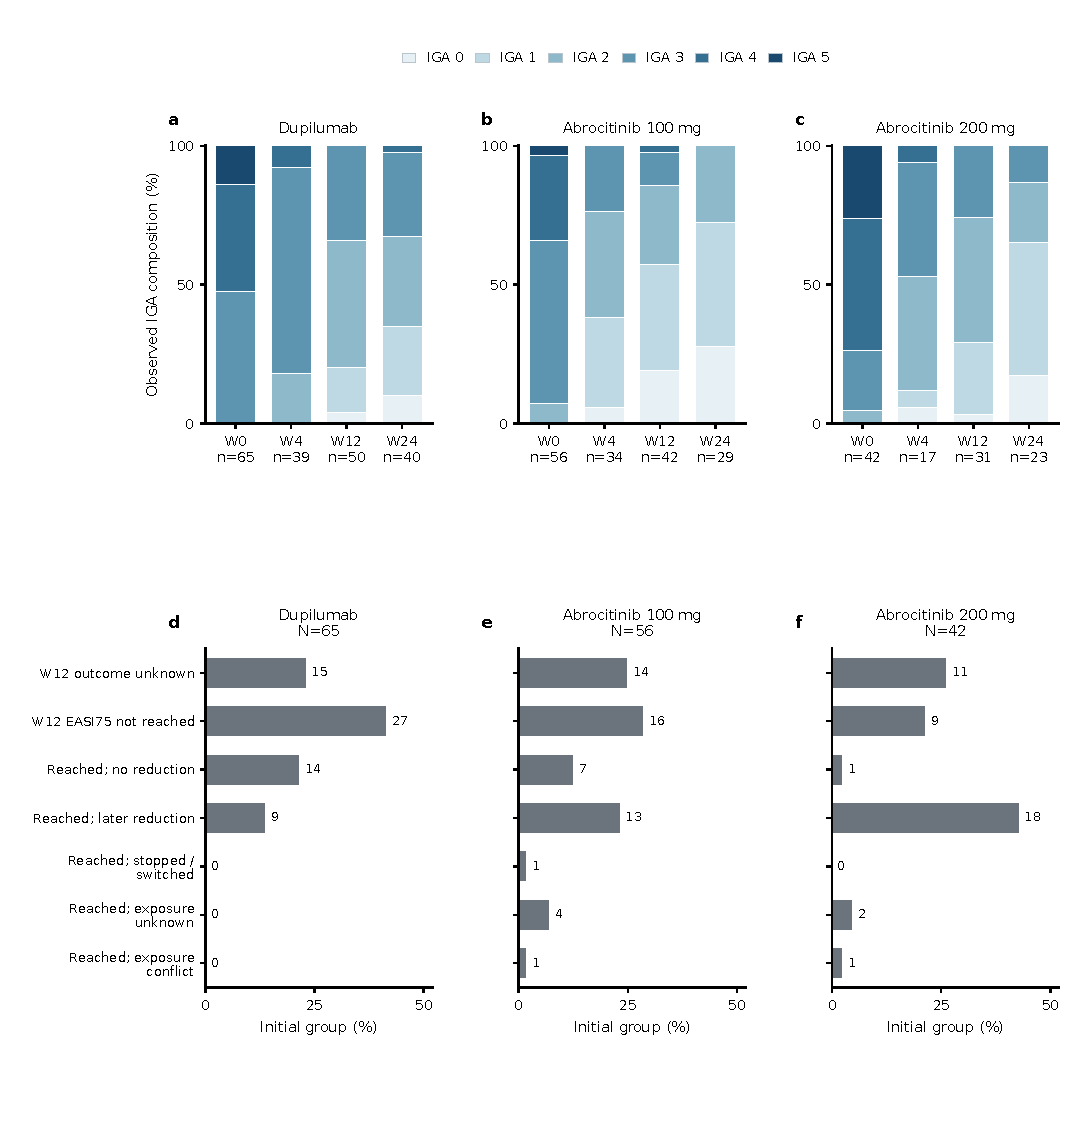
\includegraphics[width=\linewidth,height=.72\textheight,keepaspectratio]{figures/Figure3.pdf}
\caption{\textbf{Molecular response across treatments and the three-marker input panel.} a, Mean paired log$_2$ concentration changes among each marker/treatment-specific fixed set with measurements at W0, W12 and W24. W0 is the zero reference; the two displayed columns per treatment show change to W12 and W24. b, All specified between-treatment contrasts for W0--W12 from HC3-robust linear models, adjusted for starting molecular concentration, W0 EASI, age, BMI, sex and centre; dots denote the declared FDR-adjusted q<0.05. These use all eligible two-visit pairs, a different population from panel a. D, dupilumab; A100/A200, initial abrocitinib dose; pooled A, the observed mixture of the two doses. Both heatmaps use the same signed log$_2$ scale, but panel b is a difference between treatment changes, not a within-group change. Cool blue denotes a negative value, warm coral a positive value; the near-white centre is zero change/difference. Cells marked $\times$ lack an estimate. Panel a prints paired n; $\dagger$ marks fewer than five pairs; these estimates are descriptive. Each estimand has its own labelled colour bar. c--e, W0/W12/W24 paired trajectories and 95\% t confidence intervals for the three frozen model inputs. Their inclusion is based on the existing panel, not selection of significant trajectories. Exact marker-specific counts, intervals, all three windows and the complete comparison families are retained in source tables and supplementary figures.}\label{fig:Figure3}
\end{figure}

For CCL17 over W0--W12, the adjusted dupilumab-minus-A100 difference was $-1.07$ log$_2$ units (95\% CI, $-1.67$ to $-0.48$; q=0.0109). The assay-batch sensitivity estimate was $-0.72$, with an interval crossing zero (q=0.369), so this contrast was not robust to that specification. Direct adjusted contrasts, rather than separate within-group P values, addressed treatment differences. All windows and complete comparisons are retained in Supplementary Figs.~S5--S14.

Molecular and clinical changes were associated for selected marker--outcome combinations. In A100 over W0--W12, the IL-5 and PP-NRS changes had Spearman $\rho=0.742$ (31 pairs; panel-wide q=0.00156). The complete declared association family also identified TNF-$\alpha$ and TSLP changes with EASI change over W0--W24. Their descriptive response-category profiles are shown in Supplementary Fig.~S41, alongside the full-panel response-depth results in Supplementary Figs.~S26--S33. These categories are ordered clinical-improvement groups, not time points or independent validation samples.

The fixed-patient IgE check used the same 11/9/10 patients across W0/W12/W24 (Supplementary Fig.~S20). It showed decreasing group medians despite differences in the visit-level summaries, illustrating sensitivity to sample composition without proving its cause. Dupilumab W4 eosinophil observations were absent; no W4 value was interpolated. These analyses distinguish a broad molecular response from the narrower task of estimating an EASI value with three markers.

\subsection{The common-model procedure estimated follow-up EASI closely}
The model dataset contained 316 complete-input visits from 160 patients: 152 at baseline, 89 at week 12 and 75 at week 24. Development used 241 baseline/week-12 visits from 156 patients. The final equation combined BSA with CCL17, CCL26 and IL-5 through the same calculation before and during treatment. It required no treatment label, visit week or previous score (Fig.~\ref{fig:Figure4}).

Under nested patient-level validation, MAE was 3.19 at baseline (95\% CI, 2.75--3.70), 1.30 at week 12 (0.96--1.71) and 1.19 at week 24 (0.89--1.53). Spearman correlations were 0.918, 0.927 and 0.904, and concordance correlations were 0.910, 0.900 and 0.869 (Table~\ref{tab:model}). Mean signed errors at W12/W24 were +0.82/+0.84 EASI points, and calibration slopes were 0.81 (95\% CI, 0.66--0.94) and 0.73 (0.59--0.82), indicating residual overestimation and scale miscalibration. The cumulative error distributions show that 41.8\%, 84.3\% and 82.0\% of predictions, respectively, were within two EASI points. These are proportions of individual predictions, not agreement between group means.

\begin{table}[!htbp]
\centering\small
\caption{Primary performance of the common-model development procedure and matched controls.}\label{tab:model}
\begin{tabular}{lrrr}\toprule
 & W0 & W12 & W24 \\ \midrule
Patients & 152 & 89 & 75 \\ 
MAE (95\% CI) & $3.19$ ($2.75$, $3.70$) & $1.30$ ($0.96$, $1.71$) & $1.19$ ($0.89$, $1.53$) \\ 
BSA-only area MAE & 3.12 & 1.18 & 1.02 \\ 
Three-marker-only MAE & 7.63 & 7.57 & 8.69 \\ 
\shortstack[l]{Primary minus BSA-only area\\MAE difference (95\% CI)} & $0.07$ ($-0.03$, $0.17$) & $0.12$ ($0.04$, $0.20$) & $0.17$ ($0.11$, $0.24$) \\ 
RMSE & 4.45 & 2.29 & 1.87 \\ 
Mean signed error & $-0.59$ ($-1.27$, $0.07$) & $0.82$ ($0.43$, $1.29$) & $0.84$ ($0.50$, $1.25$) \\ 
Spearman correlation & 0.918 & 0.927 & 0.904 \\ 
Concordance correlation & 0.910 & 0.900 & 0.869 \\ 
Within two points, \% & 41.8 & 84.3 & 82.0 \\ 
Severity-band agreement, \% & 83.2 & 88.2 & 92.7 \\ 
\bottomrule\end{tabular}
\par\small\raggedright W0/W12 use patient-grouped nested validation; W24 is same-cohort temporal application. Structure and penalty selection are internal to each training fold; earlier marker-panel selection is not repeated. Matched controls use the same patients and outer folds. BSA-only area uses the zero-intercept area structure; three-marker-only uses CCL17, CCL26 and IL-5 without BSA. Positive paired MAE differences mean greater primary-procedure error. Metrics are averaged after scoring each repetition. Intervals are 95\% patient-bootstrap intervals conditional on saved predictions; selection and fitting are not repeated. MAE, mean absolute error; RMSE, root mean squared error. Positive signed error indicates overestimation. Severity-band agreement uses four EASI bands for observed and predicted values: $\leq7$, $>7$ to $\leq21$, $>21$ to $\leq50$, and $>50$. The single final formula is not independently validated.\end{table}

\begin{figure}[!htbp]
\centering
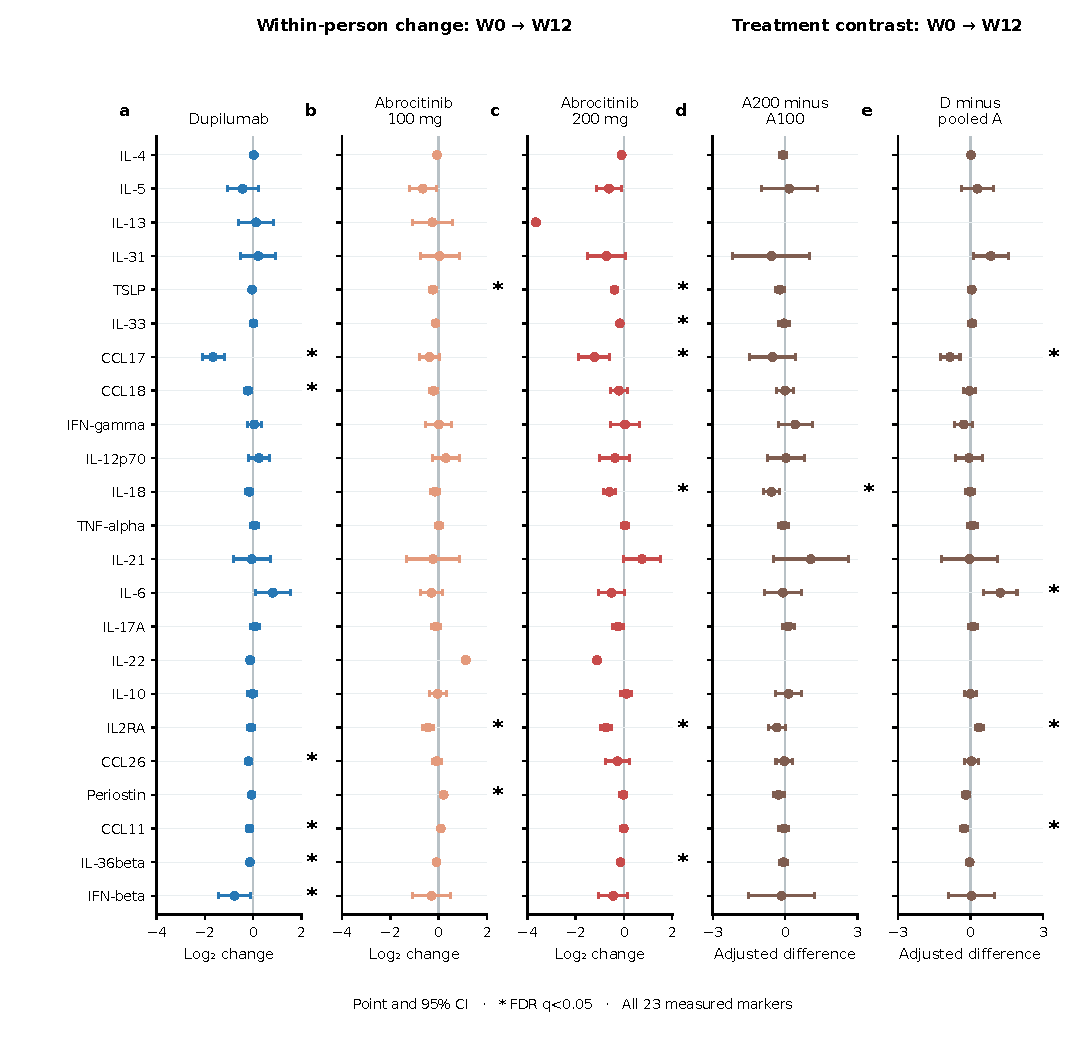
\includegraphics[width=\linewidth,height=.72\textheight,keepaspectratio]{figures/Figure4.pdf}
\caption{\textbf{Individual EASI estimation and its severity boundary.} a--c, Estimated versus observed EASI in the first patient-held-out repetition at W0/W12 and same-cohort temporal application at W24. Each fixed 2$\times$2-EASI-point cell contains all patients whose exact score pair falls within its boundaries. Colour gives patient count on the shared logarithmic count scale; white cells have no observations. All 152/89/75 eligible patients are retained, and identical axes preserve the severity-range comparison. Grey lines denote exact agreement, not a fitted association. d, Cumulative absolute-error proportions, calculated separately in each validation repetition and then averaged. Bands are patient-bootstrap 95\% confidence intervals conditional on saved predictions. All errors enter each proportion; only thresholds from zero to ten points are displayed. The two-point line is a reading reference, not an accepted replacement margin. e, Baseline MAE by observed EASI stratum, with patient-bootstrap 95\% confidence intervals and unique-patient counts. These estimates average the two repetition-specific metrics. W12/W24 have only one/no EASI>21 observation, respectively. W0/W12 use nested patient-level structure and penalty selection; earlier marker selection is not repeated. W24 was previously inspected within the same cohort. These results assess the development procedure, not independent validation of the final formula. Primary overall metrics and numerical controls appear in Table 2; molecular added accuracy has not been established.}\label{fig:Figure4}
\end{figure}

Baseline severe disease remained the principal accuracy boundary: MAE was 5.38 among the 44 patients with EASI $>21$, compared with 1.15 and 2.55 in the two lower strata (Supplementary Fig.~S35). There was only one such severe observation at week 12 and none at week 24. Centre and treatment holdouts also showed variation (Supplementary Fig.~S21). Matched BSA-area control MAEs were 1.18 and 1.02 at W12/W24, compared with 1.30 and 1.19 for the primary procedure. Paired excess errors were 0.12 points (95\% CI, 0.04--0.20) and 0.17 (0.11--0.24), conditional on saved predictions. Thus, adding the serum inputs did not improve current EASI estimation in this evaluation. Complete serum-only and fixed-structure controls remain in the source tables.

Removing eight W0 and two W12 reference-inconsistent visits from training, while retaining the original folds and evaluation outcomes, gave sensitivity MAEs of 3.19/1.15/1.06 at W0/W12/W24. This refit improved follow-up error but did not establish molecular added accuracy over the identically refitted BSA-area control. Follow-up calibration slopes remained below one. The frozen primary equation and primary estimates were retained (Supplementary Table~S4).

Independent models for PP-NRS, adult DLQI and recorded ordinal IGA did not reproduce the EASI performance with this restricted input panel. Week-12/week-24 MAEs were 2.78/2.53 for PP-NRS and 5.90/6.28 for DLQI; exact IGA agreement was 35.4\%/28.0\% (Supplementary Fig.~S34).

\subsection{The equation tracked within-person change with window-dependent precision}
Estimated and observed EASI changes followed similar ordering across all three paired intervals (Fig.~\ref{fig:Figure5}). Change MAEs were 3.87 for baseline--week 12 (85 patients; 95\% CI, 3.08--4.70), 3.47 for baseline--week 24 (67 patients; 2.68--4.39) and 1.49 for weeks 12--24 (55 patients; 1.00--2.19). The corresponding Spearman correlations were 0.873, 0.940 and 0.900. The two intervals beginning at baseline retained larger errors despite their high correlations; estimation of the baseline score contributed to this difference.

\begin{figure}[!htbp]
\centering
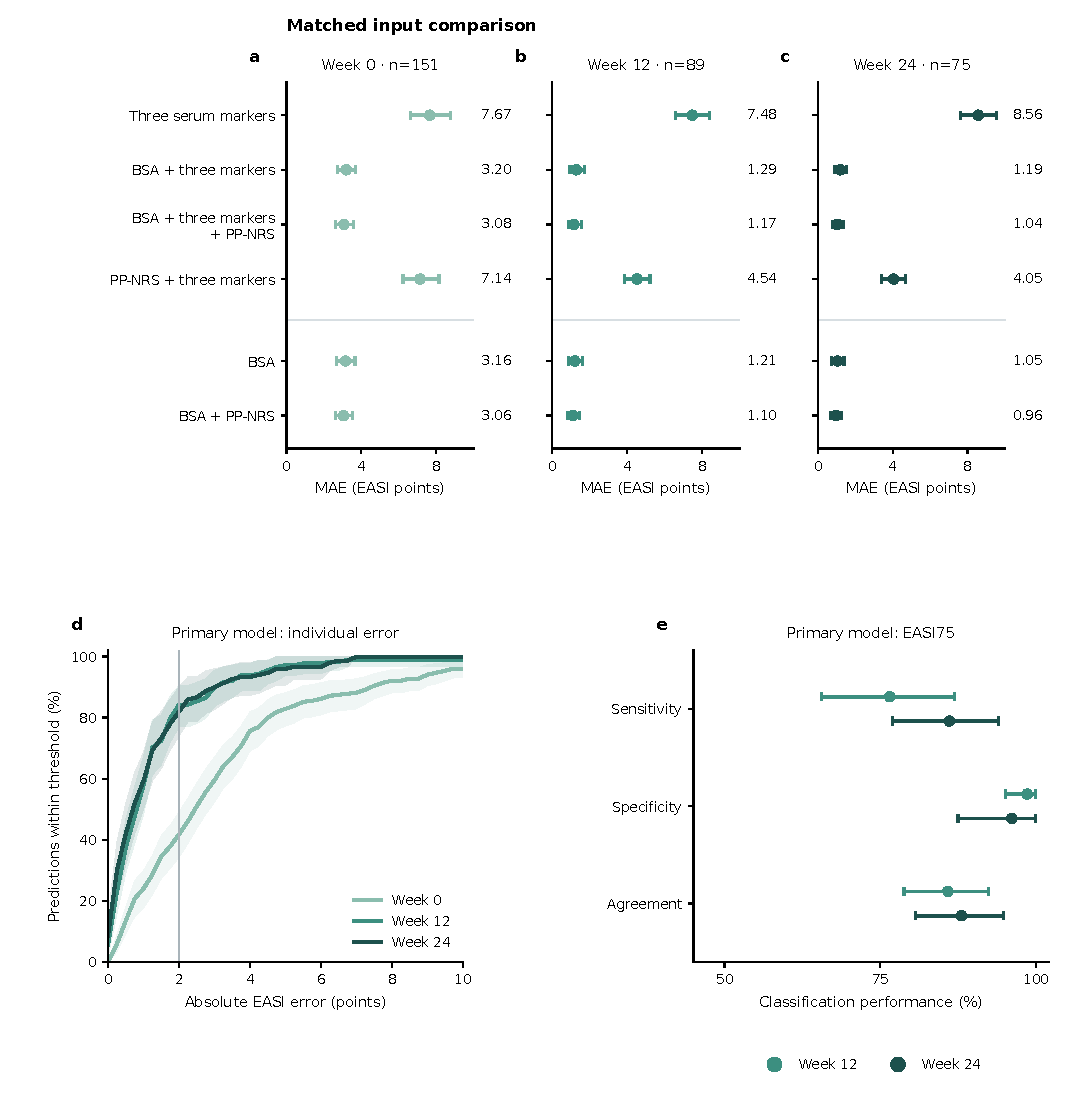
\includegraphics[width=\linewidth,height=.72\textheight,keepaspectratio]{figures/Figure5.pdf}
\caption{\textbf{Within-patient change and EASI75 response classification.} a--c, Estimated versus observed EASI changes in the first patient-held-out repetition. Change is end minus start, so negative values indicate improvement. Fixed 2$\times$2-EASI-point cells count exact paired score changes, using one logarithmic count scale and identical axes across intervals; white cells contain no observations. All 85, 67 and 55 paired patients are retained in their respective windows, which can share patients. Grey diagonal lines denote exact agreement; horizontal and vertical lines mark no change. Primary change MAEs over W0--W12, W0--W24 and W12--W24 are 3.87, 3.47 and 1.49 points, respectively, with intervals in the source tables. These metrics score each of two repetitions before averaging, whereas the count maps illustrate one repetition. d, EASI75 sensitivity, specificity and overall agreement, averaged after classification within each repetition, with patient-bootstrap 95\% confidence intervals conditional on saved predictions. Sensitivity denominators are observed responders (W12 n=49; W24 n=54); specificity denominators are nonresponders (36 and 13). Agreement includes 85 and 67 patients. Observed and estimated response each use their corresponding W0 and follow-up scores; percentage response requires positive observed and estimated W0. W24 is previously inspected same-cohort temporal application, not external validation. Complete EASI50/75/90 classifications and exclusions remain in the supplement. These results assess monitoring agreement, not treatment causality or clinical interchangeability.}\label{fig:Figure5}
\end{figure}

Using estimated scores at both visits to identify EASI75 gave sensitivities of 76.5\% at week 12 (95\% CI, 65.6--87.0) and 86.1\% at week 24 (76.9--94.0), with specificities of 98.6\% (95.2--100) and 96.2\% (87.5--100). Only 36 and 13 observed nonresponders informed specificity at the two visits. Some observed responders were missed despite the high specificity. Sensitivity for the deeper EASI90 response was lower, at 63.0\% and 52.9\% (Supplementary Fig.~S36). These separate paired evaluations support assessment of change alongside the absolute reading; they do not establish a universally interchangeable measure of treatment response.

\section{Discussion}
A common four-input model-development procedure connected nominal-visit-matched affected skin area and serum measurements to EASI throughout this Chinese treatment cohort. Its strongest performance was in follow-up disease activity, where most estimates were within two EASI points. Using the same calculation across visits also allowed changes to be expressed directly in EASI units. This makes the formula straightforward to examine and reproduce: the research equation takes BSA and three serum concentrations without a treatment label or previous score. Same-day clinical/serum matching was not verified, so its use as a contemporaneous clinical measurement requires a defined sampling window.

The equation combines two aspects of disease that have different clinical roles. BSA represents the extent of visible lesions, an established component of EASI.\citep{hanifin2022,home_easi} The molecular term adjusts that extent-based estimate using serum measurements. The full 23-marker analysis places those inputs within treatment-dependent inflammatory changes, rather than treating them as an exhaustive map of disease biology. Coefficient signs describe conditional prediction in this dataset; the negative IL-5 term, for example, is not evidence of a protective effect. The primary follow-up procedure had slightly greater error than the matched BSA-area control. Reference-consistency refitting reduced follow-up error, but still did not establish an accuracy benefit from the serum panel. The biological findings therefore give context for these inputs rather than a demonstrated reason to order the assays for EASI estimation. A future demonstration of molecular value would need independent evidence, such as explaining clinically adjudicated blood--skin discordance or anticipating a later outcome beyond the current EASI score.

Individual monitoring is a distinct test from agreement at a single visit. The formula reproduced much of the ordering of clinical improvement, yet changes beginning at baseline were less precise than later follow-up changes. Higher observed baseline severity was associated with larger errors. Severity mix, prior treatment and reference quality cannot be separated as causes by these data. Lesion intensity can vary despite similar affected area. Chinese serum endotypes and recent severity-linked proteomic findings also show broader inflammatory and epithelial-associated heterogeneity than a three-marker panel can represent.\citep{wu2023,lally2026} These observations motivate testing additional lesion information in severe disease, but they do not identify the cause of individual errors or establish that more blood markers will reduce them.

The p-EASI studies provide the closest precedent for a usable serum-to-EASI calculation.\citep{thijs2017,thijs2019,bakker2020} Their correlations and classification results encouraged molecular estimation; the present study adds explicit absolute errors, their distribution and within-person response checks in a local treatment cohort. Their use of serum alone differs from the present BSA--serum inputs. Measurement procedures can affect calibration, and both assay compatibility and case mix matter when moving a prediction rule between settings.\citep{luijken2020,riley2024validation} The source-table local-application analyses therefore provide neither a fair superiority test nor evidence that population ethnicity explains a performance difference.

Treatment context matters both for interpreting biomarkers and for comparing clinical outcomes. Patients receiving the higher initial abrocitinib dose had greater starting severity; subsequent reductions were selected after clinical response. Baseline adjustment and explicit maintenance pathways therefore address different questions. This distinction is consistent with randomized abrocitinib induction/withdrawal designs and observational dupilumab tapering studies, which define eligibility for maintenance or reduction before evaluating its success.\citep{blauvelt2022regimen,spekhorst2023} The present results describe adjusted initial-strategy associations and observed later management, rather than the effect of assigning each patient an alternative dose. Differential missingness, endpoint-specific residual imbalance and response-selected follow-up limit these comparisons even after baseline adjustment. They also preserve itch and quality-of-life outcomes as complementary clinical domains; neither is adequately recovered by the same small serum--BSA panel.

The proposed management concept keeps the research EASI estimate alongside measured skin findings, symptoms, quality of life and safety (Fig.~\ref{fig:Figure1}). It does not supply automatic escalation, reduction or stopping thresholds. Independent evaluation should test the frozen equation, assay procedure and a prespecified clinical decision together. Patient-level validation prevented a person's repeated visits from appearing in both training and testing, but the molecular panel had been selected earlier and week 24 had already been inspected in prior project analyses. The current evidence consequently supports within-cohort performance of the development procedure, with a clearly defined research formula for the next evaluation. Patient bootstrap intervals condition on saved predictions and omit model-development uncertainty; no independent validation of the single final formula has been performed. Follow-up overestimation and calibration slopes below one also argue against substituting estimates for clinical examination. Adequate numbers of active severe cases, independent clinical assessment and a prespecified tolerance for individual errors will determine whether the same simple calculation can support decisions across the full disease range.

\section*{Data and code availability}
Analysis code, versioned parameters, aggregate source tables and figure sources are available at \url{https://github.com/yanax726/T2T}. Figures and tables can be rebuilt from aggregates; model refitting requires the declared restricted input snapshots. Patient-level clinical records, serum measurements, dates and free-text notes are not included in the public repository. Access conditions and the institutional contact for these restricted records require author confirmation.
\bibliographystyle{unsrtnat}
\bibliography{references}
\end{document}
